\documentclass[tikz]{standalone}

\usepackage{amsmath}
\usepackage{circuitikz}

\usetikzlibrary{positioning}

\let\Re\undefined
\let\Im\undefined
\DeclareMathOperator{\Re}{\operatorname{Re}}
\DeclareMathOperator{\Im}{\operatorname{Im}}

\begin{document}
	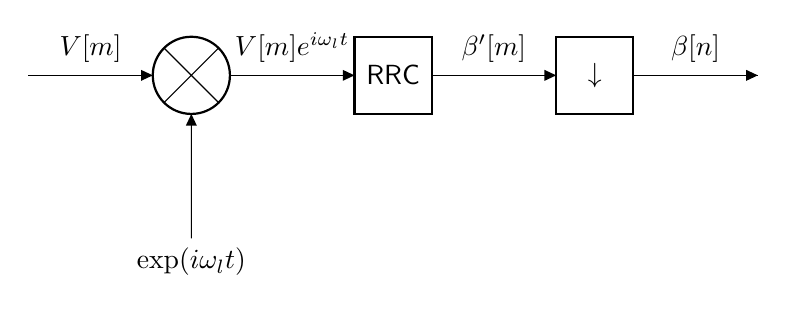
\begin{tikzpicture}[
		node distance=4.5em,
	]
		\coordinate (in) at (0,0);
		\node [mixer, right=of in] (mixer) {};
		\node [twoportshape, t=\sffamily{RRC}, right=of mixer] (rrc) {};
		\node [twoportshape, t=$\downarrow$, right=of rrc] (dwn) {};
		\coordinate[right=of dwn] (out);
		\node [below=of mixer] (osc) {$\exp(i\omega_lt)$};
		
		\draw (in) to[short, l={$V[m]$}] (mixer.west) node[inputarrow]{};
		\draw (mixer.east) to[short, l={$V[m]e^{i\omega_lt}$}] (rrc.west) node[inputarrow]{};
		\draw (rrc.east) to[short, l={$\beta^\prime[m]$}] (dwn.west) node[inputarrow]{};
		\draw (dwn.east) to[short, l={$\beta[n]$}] (out) node[inputarrow]{};
		\draw (osc) to[short] (mixer.south) node[inputarrow, rotate=90]{};
	\end{tikzpicture}
\end{document}
